% !TeX program = xelatex
% Name: Thiều Quang
% ID: 24127114
% Member: Tôn Thất Việt Khoa
% ID: 24127190
% Course: Khai thác dữ liệu và ứng dụng (Data Mining and Applications)
% Assignment: https://hcmus-cs-ta.github.io/lab-book/data-mining/projects/itemset/
% IEEE Conference two-column layout, source text in Vietnamese.
\documentclass[conference,10pt]{IEEEtran}
\usepackage{fontspec}
% Times New Roman and Arial are used on Windows; portable fallbacks allow XeLaTeX elsewhere.
\IfFontExistsTF{Times New Roman}{\setmainfont{Times New Roman}}{\setmainfont{Liberation Serif}}
\IfFontExistsTF{Arial}{\setsansfont{Arial}}{\setsansfont{Liberation Sans}}
\usepackage{amsmath,amssymb,booktabs,array,graphicx,multirow}
\usepackage{tikz}
\usetikzlibrary{positioning}
\usepackage[hidelinks]{hyperref}
\usepackage{url}
\usepackage{enumitem}
\usepackage{microtype}
\usepackage{fancyhdr}
\usepackage{placeins}
\usepackage{balance}
\setlength{\parindent}{1em}
\setlength{\parskip}{0pt}
\raggedbottom
% Allow related tables to share a float page instead of being flushed one by one.
\makeatletter
\setlength{\@fptop}{0pt}
\setlength{\@fpsep}{12pt plus 2pt minus 2pt}
\setlength{\@dblfptop}{0pt}
\setlength{\@dblfpsep}{12pt plus 2pt minus 2pt}
\makeatother
\newcommand{\myitem}[1]{\texttt{#1}}
\title{Khai thác tập mục phổ biến bằng Eclat: Cài đặt độc lập, thiết kế thực nghiệm và hai ứng dụng thực tế\\[2mm]
\large Báo cáo thực nghiệm}
\author{
\IEEEauthorblockN{%
\begin{tabular}{@{}c@{\hspace{18mm}}c@{}}
Thiều Quang & Tôn Thất Việt Khoa\\
{\normalfont\small MSSV: 24127114} & {\normalfont\small MSSV: 24127190}
\end{tabular}}
\IEEEauthorblockA{Trường Đại học Khoa học Tự nhiên, ĐHQG-HCM\\Học phần: Khai thác dữ liệu và ứng dụng\\(Data Mining and Applications)}
}
\begin{document}
\maketitle
\begin{abstract}
Báo cáo trình bày hai bản cài đặt độc lập của Eclat bằng Python và Julia, mỗi bản có hai cách lưu TID-set. Bản Python đạt 41/41 ca pytest và 48/48 lượt benchmark trên bốn bộ dữ liệu. Bản Julia 1.13.3 đạt 77/77 phép kiểm thử và 48/48 lượt benchmark; toàn bộ 24/24 cấu hình được đối chiếu trùng từng itemset và support với SPMF trên Windows. Python cũng khớp 25/25 trường hợp, gồm dữ liệu toy, khi chạy trên Google Colab. Với BMS\_WebView\_1, SPMF sử dụng ánh xạ tạm ID mà không sửa tập dữ liệu gốc. Hai ứng dụng gồm khai thác giỏ hàng và các mẫu thị giác từ 600 ảnh chữ số. Báo cáo nêu rõ giới hạn khi so sánh thời gian giữa các môi trường và phương pháp đo khác nhau.
\end{abstract}
\begin{IEEEkeywords}
Eclat; frequent itemset mining; vertical database; bitset; market basket analysis; bag of visual words; reproducibility.
\end{IEEEkeywords}

\section{Giới thiệu và phạm vi nghiên cứu}
Các hệ thống bán lẻ, nền tảng nội dung và xử lý dữ liệu ảnh thường tạo ra lượng lớn bản ghi có thể biểu diễn thành tập các phần tử rời rạc. Trong bài toán FIM, một mẫu là \emph{tập mục} được quan sát cùng nhau với tần suất không nhỏ hơn ngưỡng quy định. Khai thác được các mẫu này có thể hỗ trợ đề xuất hàng hóa, mô tả đồng xuất hiện của hoạt động hoặc khám phá nhóm đặc trưng thị giác. Phương pháp cổ điển Apriori tổ chức tìm kiếm theo số lượng phần tử trong mẫu; Eclat chuyển trọng tâm sang giao các danh sách giao dịch chứa từng mục, cùng chiến lược tìm kiếm theo chiều sâu \cite{zaki2000,agrawal1994}.

Bài thực hành đặt yêu cầu tự cài đặt một thuật toán FIM, kiểm chứng với SPMF, thực nghiệm trên ít nhất bốn cơ sở dữ liệu và triển khai hai ứng dụng có bước chuyển dữ liệu thành giao dịch \cite{assignment}. Nhóm tự triển khai Eclat bằng Python và Julia; mã nguồn tham chiếu SPMF được tách khỏi mã khai thác, dữ liệu nguồn và chương trình thử nghiệm. SPMF được sử dụng trong giai đoạn đánh giá đầu ra, không phải đầu vào cho việc phát triển thuật toán.

\subsection{Câu hỏi nghiên cứu}
Ba câu hỏi được đặt ra: (1) cài đặt Eclat độc lập có tìm đúng mọi itemset và support tuyệt đối hay không; (2) khác biệt giữa TID-set thông thường và bitset ảnh hưởng thời gian/bộ nhớ như thế nào trên dữ liệu dày và thưa; (3) phép biến đổi từ giao dịch bán lẻ hoặc ảnh số sang biểu diễn tập hợp giữ được những tín hiệu hữu ích nào và đánh mất thông tin gì.

\subsection{Phạm vi và giới hạn}
Eclat được chọn là \emph{duy nhất} trong nhóm vertical FIM; dEclat là một biến thể liên quan nhưng không được cài đặt trong đề tài này. Mẫu được xem là \emph{unordered}: không quan tâm thứ tự các mục và không giữ số lần một mục lặp trong cùng giao dịch. Với ứng dụng ảnh, mỗi visual word xuất hiện một lần về mặt tập hợp, bất kể số patch được gán vào cụm tương ứng. Báo cáo sử dụng các benchmark đã tải từ SPMF, đồng thời đánh giá tính đúng đắn thông qua kết quả đối chiếu với SPMF độc lập.

\section{Phát biểu bài toán và cơ sở toán học}
Cho tập mục hữu hạn $I=\{i_1,\dots,i_m\}$, cơ sở dữ liệu giao dịch $D=(T_1,\dots,T_n)$, $T_j\subseteq I$. Mỗi $T_j$ mang một chỉ số giao dịch $j$ duy nhất. Đối với $X\subseteq I$, \emph{support count} được định nghĩa như trong (1):
\begin{equation}\label{eq:supportcount}
\sigma_D(X)=\big|\{j\in\{1,\dots,n\}:X\subseteq T_j\}\big|.
\end{equation}
\emph{Relative support} là $\mathrm{sup}_D(X)=\sigma_D(X)/n$. Với ngưỡng $s\in(0,1]$, itemset $X$ phổ biến nếu $\sigma_D(X)\ge\lceil sn\rceil$. Nếu ngưỡng được nhập dưới dạng số nguyên $k\ge1$, điều kiện trở thành $\sigma_D(X)\ge k$. Cần phân biệt hai trường hợp này vì thay đổi quy ước có thể làm kết quả lệch so với phần mềm tham chiếu.

\subsection{Tính đơn điệu nghịch của support}
Nếu $X\subseteq Y$ thì mọi giao dịch chứa $Y$ cũng chứa $X$; từ đó $\sigma_D(Y)\le\sigma_D(X)$. Hệ quả: khi $X$ không phổ biến, mọi siêu tập của $X$ cũng không phổ biến. Đây là nguyên lý tỉa nhánh cơ bản. Nó giải thích vì sao tìm kiếm không nhất thiết phải liệt kê đủ $2^{m}-1$ tập con trong mọi tình huống. Tuy vậy, khi bản thân số itemset phổ biến quá lớn, bất kỳ thuật toán xuất đầy đủ kết quả nào cũng phải chịu chi phí đầu ra tương ứng.

\subsection{Cách nhìn theo TID-set}
Định nghĩa $\mathrm{tid}(X)=\{j:X\subseteq T_j\}$. Khi đó $\sigma_D(X)=|\mathrm{tid}(X)|$ và
\begin{equation}\label{eq:tidintersection}
\mathrm{tid}(X\cup Y)=\mathrm{tid}(X)\cap\mathrm{tid}(Y).
\end{equation}
Đồng nhất thức (2) cho phép tính support của itemset lớn hơn bằng cách giao TID-set mà không cần quét tất cả giao dịch gốc cho mỗi ứng viên. Dữ liệu được chuyển từ biểu diễn theo hàng sang biểu diễn theo cột: mỗi item dẫn tới tập các giao dịch xuất hiện nó.

\begin{table}[t]
\centering\caption{Ví dụ giao dịch tự tạo dùng minh họa; không phải benchmark}\label{tab:toy}
\begin{tabular}{@{}ll@{}}\toprule
TID & Tập mục\\\midrule
1 & $\{1,2,3\}$\\
2 & $\{1,2\}$\\
3 & $\{1,3\}$\\
4 & $\{2,3\}$\\
5 & $\{1,2,3\}$\\
6 & $\{2\}$\\\bottomrule
\end{tabular}
\end{table}

Theo Bảng~\ref{tab:toy}, $\mathrm{tid}(1)=\{1,2,3,5\}$ và $\mathrm{tid}(2)=\{1,2,4,5,6\}$. Phép giao cho $\mathrm{tid}(\{1,2\})=\{1,2,5\}$, tức support count bằng $3$ và relative support bằng $0.5$. Với minsup $0.5$, itemset $\{1,2\}$ là phổ biến.

\section{Tổ chức dữ liệu theo chiều dọc và phép giao}
Trong cấu trúc cơ bản, một từ điển ánh xạ item sang \myitem{set[int]} giao dịch. Tập ID được giữ theo thứ tự tùy ý nhưng phép toán giao trong Python trả về đúng tập phần tử chung. Phiên bản tối ưu dùng một số nguyên lớn $b_i$ cho mỗi item $i$, trong đó bit thứ $j$ có giá trị $1$ nếu và chỉ nếu giao dịch $j$ chứa item. Với hai mục $i$ và $k$, phép giao được thay bằng $b_i\mathbin{\&}b_k$; số bit một cho biết support. Các phép toán này sử dụng mã máy và tránh cấp phát nhiều đối tượng số nguyên trong mỗi TID-set con, nhưng không bảo đảm luôn tốt hơn trên mọi cơ sở dữ liệu.

\begin{equation}\label{eq:bits}
 b_X=\bigwedge_{i\in X}b_i,\qquad \sigma_D(X)=\mathrm{popcount}(b_X).
\end{equation}
Ký hiệu $\wedge$ chỉ phép AND bit; $\mathrm{popcount}$ đếm số bit bằng $1$. Python cung cấp phép \myitem{int.bit\_count()} để thực hiện thao tác sau. Cả hai biến thể đều xuất danh sách itemset với support tuyệt đối, không áp dụng xấp xỉ.

\begin{figure}[t]
\centering
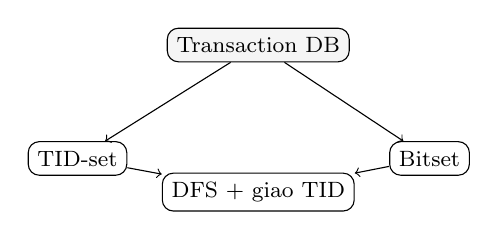
\begin{tikzpicture}[node distance=10mm, every node/.style={font=\footnotesize}]
\node[draw,rounded corners,fill=gray!8] (tr) {Transaction DB};
\node[draw,rounded corners,below left=10mm and 5mm of tr] (s) {TID-set};
\node[draw,rounded corners,below right=10mm and 5mm of tr] (b) {Bitset};
\node[draw,rounded corners,below=14mm of tr] (dfs) {DFS + giao TID};
\draw[->] (tr) -- (s);\draw[->] (tr) -- (b);
\draw[->] (s) -- (dfs);\draw[->] (b) -- (dfs);
\end{tikzpicture}
\caption{Sơ đồ hai biểu diễn dữ liệu trong cùng một thuật toán Eclat.}\label{fig:architecture}
\end{figure}

Hình~\ref{fig:architecture} cho thấy việc lựa chọn kiểu lưu trữ không làm thay đổi ngữ nghĩa của Eclat. Mã nguồn nằm ở \myitem{src/algorithm/eclat.py}; \myitem{src/structures.py} mô tả cấu trúc dữ liệu, còn \myitem{src/utils.py} tách thao tác I/O. Trình biên dịch Python chuẩn và thư viện hệ thống đủ chạy thuật toán; NumPy chỉ cần cho bước lượng tử hóa đặc trưng ảnh ở ứng dụng thứ hai.

\subsection{Bản cài đặt Eclat bằng Julia}
Bên cạnh Python, project có mô-đun \myitem{julia/EclatJulia.jl} sử dụng hai backend \myitem{Set} và \myitem{BitVector}. Cả hai đều xây dựng cơ sở dữ liệu dọc, giao các TID-set theo tìm kiếm chiều sâu và trả về cùng ánh xạ itemset--support. Với \myitem{BitVector}, phép giao được thực hiện bằng AND trên vector bit, còn support là số bit được bật; cách cài đặt này độc lập với kiểu số nguyên bitset trong Python.

Giao diện dòng lệnh \myitem{julia/main.jl} nhận \myitem{--input}, \myitem{--minsup}, \myitem{--output} và \myitem{--backend}; đầu ra dùng định dạng \myitem{\#SUP:} tương thích SPMF. Trên Windows, Julia 1.13.3 vượt qua 17 phép kiểm thử chức năng và 60 phép so sánh với brute force, tổng cộng 77/77. Trên bốn bộ dữ liệu benchmark, cả 48 lượt theo hai backend đều đạt kiểm tra nhất quán; 24/24 cặp dataset--minsup khớp chính xác toàn bộ itemset và support với SPMF. Các số liệu này là kết quả của lần chạy đã được ghi nhận, không phải ước lượng từ đồ thị.

\section{Thủ tục Eclat và tính đúng đắn}
Eclat xây dựng danh sách các item phổ biến đơn, sắp theo một thứ tự xác định để tránh sinh cùng tập mục nhiều lần. Trong mỗi lời gọi đệ quy với tiền tố $P$, thuật toán duyệt từng phần tử mở rộng $x$ có TID-set tương ứng, ghi nhận $P\cup\{x\}$ và sinh tiếp các mở rộng theo các mục còn lại có thứ tự phía sau $x$. Một nhánh chỉ được mở khi giao TID-set vẫn đạt ngưỡng support. Mỗi tập mục có một dãy mục tăng dần duy nhất theo thứ tự đã chọn; do đó không trùng lặp output. Trật tự này chỉ nhằm tổ chức tìm kiếm, không phải thứ tự của items trong từng giao dịch.

\subsection{Phác thảo mã giả}
\noindent\textbf{Đầu vào:} danh sách $(i,\mathrm{tid}(i))$ đã lọc phổ biến; tiền tố $P$.\\
\textbf{Bước 1:} chọn lần lượt cặp $(i,U)$ trong phần đuôi.\\
\textbf{Bước 2:} ghi $P\cup\{i\}$ với support $|U|$.\\
\textbf{Bước 3:} với mục $j$ còn lại, tính $V=U\cap\mathrm{tid}(j)$; nếu $|V|\ge\text{minsup}_{abs}$ thì giữ lại làm mở rộng.\\
\textbf{Bước 4:} gọi đệ quy trên $P\cup\{i\}$ với phần đuôi mới.\\
\textbf{Dừng:} khi không có mục mở rộng đạt ngưỡng.

\subsection{Lập luận đúng đắn}
\textit{Tính đúng}: Mỗi itemset được ghi nhận từ một giao TID-set đúng theo (2); điều kiện ngưỡng áp dụng trực tiếp lên số giao dịch chứa đủ các mục. Không có itemset thiếu support được xuất. \textit{Tính đầy đủ}: với một tập phổ biến $X$, mọi tiền tố theo thứ tự mở rộng đều là tập con của $X$ nên phổ biến; vì thế nhánh tương ứng không bị tỉa. Lần lượt mở rộng các phần tử của $X$ sẽ đến đúng nút sinh $X$. \textit{Không trùng}: thứ tự mở rộng chỉ chọn những phần tử đứng sau nút hiện tại, nên hai hoán vị của cùng một tập không thể tạo hai đường đi.

\subsection{Độ phức tạp và điểm nghẽn}
Trong trường hợp xấu nhất, có thể có tới $2^m-1$ itemset phổ biến; tổng chi phí không thể tốt hơn kích thước đầu ra. Giao TID-set dạng set phụ thuộc vào độ lớn hai tập trung gian; dạng bitset thực hiện thao tác theo số từ máy cần lưu $n$ bit. Chi phí dựng dữ liệu theo chiều dọc tuyến tính theo tổng số lần xuất hiện item trong cơ sở dữ liệu. Không nên khẳng định từ lý thuyết rằng bitset luôn nhanh hơn, vì bitset dày đặc có thể lãng phí khi giao dịch thưa.

% Two fully worked, independently checked toy datasets for the HCMUS Eclat report.
% Item labels A,B,C,D,E correspond to integer IDs 1,2,3,4,5 in data/toy/.
\section{Hai ví dụ minh họa Eclat tính tay}
\label{sec:hand-examples}
Để kiểm tra cách Eclat tính support, phần này sử dụng hai bộ dữ liệu nhỏ \emph{tự tạo}, tách biệt hoàn toàn với bốn bộ benchmark. Quy ước $A,B,C,D,E$ tương ứng với item ID $1,2,3,4,5$. Cả hai ví dụ có sáu giao dịch, năm item và cùng ngưỡng $\mathrm{minsup}=50\%$, tức $\lceil 6\times0.5\rceil=3$ giao dịch. Khi duyệt bằng tay, các item được xét theo thứ tự $A<B<C<D<E$; thứ tự duyệt thực tế của chương trình có thể khác nhưng tập kết quả không đổi.

\subsection{Ví dụ 1: Giao TID-set và tìm đầy đủ tập phổ biến}
\noindent\textbf{Bước 1 -- Lập cơ sở dữ liệu giao dịch.} Sáu giỏ hàng tự tạo như sau:
\begin{center}
\small
\begin{tabular}{@{}cl@{}}\toprule
TID & Các item trong giao dịch\\\midrule
$T_1$ & $\{A,B,C,D\}$\\
$T_2$ & $\{A,B,C\}$\\
$T_3$ & $\{A,B,D\}$\\
$T_4$ & $\{A,C,D,E\}$\\
$T_5$ & $\{B,C,D\}$\\
$T_6$ & $\{A,B,C,E\}$\\\bottomrule
\end{tabular}
\end{center}
\noindent\textbf{Bước 2 -- Chuyển sang dữ liệu dọc.} Quét sáu giao dịch một lần, ghi TID-set cho từng item:
\begin{center}
\footnotesize
\setlength{\tabcolsep}{3pt}
\begin{tabular}{@{}clrc@{}}\toprule
Item & TID-set & $\sigma$ & Giữ?\\\midrule
$A$ & $\{1,2,3,4,6\}$ & 5 & Có\\
$B$ & $\{1,2,3,5,6\}$ & 5 & Có\\
$C$ & $\{1,2,4,5,6\}$ & 5 & Có\\
$D$ & $\{1,3,4,5\}$   & 4 & Có\\
$E$ & $\{4,6\}$       & 2 & Không\\\bottomrule
\end{tabular}
\end{center}
Vì $\sigma(E)=2<3$, Eclat loại $E$ ngay tại nút gốc; các tập chứa $E$ cũng không thể phổ biến (tính đơn điệu nghịch).

\noindent\textbf{Bước 3 -- Mở rộng từ các item đơn.} Với hai item bất kỳ $X,Y$, dùng $\mathrm{tid}(XY)=\mathrm{tid}(X)\cap\mathrm{tid}(Y)$. Chẳng hạn:
\begin{equation*}
\begin{aligned}
\mathrm{tid}(AB)&=\{1,2,3,4,6\}\cap\{1,2,3,5,6\}\\
                &=\{1,2,3,6\},\qquad \sigma(AB)=4.
\end{aligned}
\end{equation*}
Thực hiện tương tự cho mọi cặp còn lại trong phần đuôi theo DFS:
\begin{center}
\footnotesize
\setlength{\tabcolsep}{4pt}
\begin{tabular}{@{}clrc@{}}\toprule
Cặp & TID-set giao & $\sigma$ & Giữ?\\\midrule
$AB$ & $\{1,2,3,6\}$ & 4 & Có\\
$AC$ & $\{1,2,4,6\}$ & 4 & Có\\
$AD$ & $\{1,3,4\}$   & 3 & Có\\
$BC$ & $\{1,2,5,6\}$ & 4 & Có\\
$BD$ & $\{1,3,5\}$   & 3 & Có\\
$CD$ & $\{1,4,5\}$   & 3 & Có\\\bottomrule
\end{tabular}
\end{center}
\noindent\textbf{Bước 4 -- Xét các nhánh độ sâu ba.} Từ nhánh $AB$, giao tiếp với $C$ và $D$:
\begin{equation*}
\begin{aligned}
\mathrm{tid}(ABC)&=\{1,2,3,6\}\cap\{1,2,4,5,6\}\\
                 &=\{1,2,6\}\ \Rightarrow\ \sigma(ABC)=3,\\
\mathrm{tid}(ABD)&=\{1,2,3,6\}\cap\{1,3,4,5\}\\
                 &=\{1,3\}\ \Rightarrow\ \sigma(ABD)=2.
\end{aligned}
\end{equation*}
$ABC$ được giữ, $ABD$ bị tỉa. Với các nhánh $AC$ và $BC$, ta có $\mathrm{tid}(ACD)=\{1,4\}$ và $\mathrm{tid}(BCD)=\{1,5\}$, đều có support $2$. Như vậy không có tập ba item nào khác đạt ngưỡng. Đặc biệt, $ABCD$ là siêu tập của $ABD$ nên không cần mở rộng sâu hơn.

\noindent\textbf{Bước 5 -- Kiểm tra lại bằng cách đếm trên dữ liệu gốc.} Bốn item đơn phổ biến có support $A:5$, $B:5$, $C:5$, $D:4$; sáu cặp có support $AB:4$, $AC:4$, $AD:3$, $BC:4$, $BD:3$, $CD:3$; một bộ ba $ABC:3$. Tổng cộng \textbf{11 frequent itemsets}. Đối chiếu trực tiếp: $ABC$ chỉ xuất hiện tại $T_1,T_2,T_6$ (ba giao dịch); $ABD$ chỉ tại $T_1,T_3$ (hai giao dịch), nên kết quả của phép giao đúng với phép đếm tay.

\subsection{Ví dụ 2: Hai item cùng TID-set và tỉa nhánh}
\noindent\textbf{Bước 1 -- Dữ liệu có trường hợp đặc biệt.} Hai item $A$ và $B$ luôn cùng xuất hiện: không có giao dịch nào chứa riêng một trong hai item.
\begin{center}
\small
\begin{tabular}{@{}cl@{}}\toprule
TID & Các item trong giao dịch\\\midrule
$T_1$ & $\{A,B,C,D\}$\\
$T_2$ & $\{A,B,C\}$\\
$T_3$ & $\{A,B,D,E\}$\\
$T_4$ & $\{A,B,C,D\}$\\
$T_5$ & $\{C,D,E\}$\\
$T_6$ & $\{C,E\}$\\\bottomrule
\end{tabular}
\end{center}
\noindent\textbf{Bước 2 -- Tính TID-set.} Từ sáu giao dịch thu được
\begin{equation*}
\begin{aligned}
\mathrm{tid}(A)&=\mathrm{tid}(B)=\{1,2,3,4\},\\
\mathrm{tid}(C)&=\{1,2,4,5,6\},\\
\mathrm{tid}(D)&=\{1,3,4,5\},\\
\mathrm{tid}(E)&=\{3,5,6\}.
\end{aligned}
\end{equation*}
Cả năm item đơn đều phổ biến, với support lần lượt là $4,4,5,4,3$. Do TID-set của $A$ và $B$ bằng nhau,
\begin{equation*}
\mathrm{tid}(AB)=\mathrm{tid}(A)\cap\mathrm{tid}(B)
=\{1,2,3,4\},\quad\sigma(AB)=4.
\end{equation*}
Đây \emph{không phải} là hai giao dịch trùng lặp: $A$, $B$ và $AB$ là ba itemset khác nhau, đều phải được xuất trong bài toán tìm \emph{tất cả} frequent itemsets.

\noindent\textbf{Bước 3 -- Mở rộng và tỉa nhánh.} Xét toàn bộ mười cặp item để không bỏ sót kết quả:
\begin{equation*}
\begin{aligned}
&AB:4,\ AC:3,\ AD:3,\ BC:3,\ BD:3,\ CD:3;\\
&AE:1,\ BE:1,\ CE:2,\ DE:2.
\end{aligned}
\end{equation*}
Sáu cặp ở dòng đầu được giữ; bốn cặp chứa $E$ có support dưới $3$ nên không mở rộng. Chẳng hạn $\mathrm{tid}(AE)=\{3\}$; vì thế $ABE$, $ACE$ và $ADE$ không cần được sinh từ nhánh $AE$.

\noindent\textbf{Bước 4 -- Xét ba item và dừng DFS.} Ta thu được
\begin{equation*}
\begin{aligned}
\mathrm{tid}(ABC)&=\{1,2,4\},\ &\sigma(ABC)&=3,\\
\mathrm{tid}(ABD)&=\{1,3,4\},\ &\sigma(ABD)&=3,\\
\mathrm{tid}(ACD)&=\{1,4\},\ &\sigma(ACD)&=2,\\
\mathrm{tid}(BCD)&=\{1,4\},\ &\sigma(BCD)&=2.
\end{aligned}
\end{equation*}
Hai tập $ABC$, $ABD$ được giữ; các nhánh $ACD$, $BCD$ bị tỉa. Tập bốn item $ABCD$ không thể phổ biến vì chứa $ACD$ không phổ biến. Các tập chứa $E$ cùng item khác cũng đã bị loại ở bước trước.

\noindent\textbf{Bước 5 -- Đối chiếu thủ công.} Danh sách đầy đủ là năm item đơn $A(4),B(4),C(5),D(4),E(3)$; sáu cặp $AB(4),AC(3),AD(3),BC(3),BD(3),CD(3)$; hai bộ ba $ABC(3),ABD(3)$. Tổng cộng \textbf{13 frequent itemsets}. Quét lại giao dịch: $AB$ xuất hiện ở $T_1,T_2,T_3,T_4$; $ABC$ ở $T_1,T_2,T_4$; $ABD$ ở $T_1,T_3,T_4$, đúng với support tính bằng TID-set. Trường hợp hai item có cùng TID-set vì vậy không làm Eclat bỏ sót hoặc ghi trùng itemset; tính đúng đắn vẫn dựa vào thứ tự mở rộng và quy tắc tỉa theo support.

Hai bộ dữ liệu tự tạo cùng danh sách itemset--support mong đợi được lưu trong thư mục \myitem{data/toy/}. Script \myitem{scripts/check\_hand\_examples.py} kiểm tra độc lập bằng cách quét lại giao dịch và liệt kê các tập con, không sử dụng lõi Eclat. Hai ví dụ chỉ nhằm minh họa cách tính tay, không thay thế kết quả 41 ca kiểm thử Python, 77 ca kiểm thử Julia hoặc các benchmark lớn.

\FloatBarrier


\section{Thiết kế kiểm thử và khả năng tái tạo}
Đề tài kiểm thử ít nhất năm cơ sở dữ liệu nhỏ khác nhau bằng một \emph{brute-force oracle} hoàn toàn độc lập với Eclat: liệt kê mọi tập con của miền item nhỏ, quét giao dịch và đếm support. Bộ oracle chỉ dùng cho dữ liệu nhỏ, không được dùng thay cho SPMF trong benchmark lớn. Các test khác kiểm tra support trên ví dụ tay, xuất/đọc định dạng \myitem{\#SUP:}, trường hợp item trùng, giao dịch rỗng, các phép kiểm tra ngưỡng và tính ổn định của codebook ảnh.

\begin{table}[t]
\centering\caption{Kết quả kiểm thử nội bộ ghi nhận trong môi trường dựng project}\label{tab:test}
\begin{tabular}{@{}p{.41\columnwidth}p{.40\columnwidth}@{}}\toprule
Hạng mục & Trạng thái\\\midrule
41 ca Pytest & Đạt 41/41 (Windows)\\
So set/bitset với brute force & Đạt (cơ sở dữ liệu nhỏ)\\
Foodmart, c20d10k, t25i10d10k & Khớp 18/18 trường hợp\\
BMS\_WebView\_1 & Khớp 6/6 trường hợp\\
Toy & Khớp\\
Julia: 77 phép kiểm thử & Đạt 77/77 (Windows)\\\bottomrule
\end{tabular}
\end{table}

Bảng~\ref{tab:test} tóm tắt kết quả kiểm thử nội bộ đã lưu trong \myitem{docs/test\_output.txt}. Kết quả 41 ca đạt phản ánh phạm vi kiểm thử ghi nhận tại thời điểm đó; không suy ra từ đây độ chính xác trên benchmark. Tính đúng được đánh giá riêng bằng kiểm thử đơn vị, nhất quán giữa hai backend và so sánh toàn bộ ánh xạ itemset--support với SPMF.

\subsection{Đầu vào, ngưỡng và đầu ra}
Mỗi dòng dữ liệu là một giao dịch gồm các item số nguyên phân tách bằng khoảng trắng. Dấu \myitem{-1}, \myitem{-2} thuộc cấu trúc chuỗi tuần tự sẽ bị từ chối, vì không phải định dạng giao dịch FIM trong đề bài. Việc gộp mục trùng là cần thiết để hỗ trợ luôn là \emph{số giao dịch} có mục, không phải số lần xuất hiện mục. File kết quả được sắp theo độ dài itemset rồi theo thứ tự ID, định dạng \myitem{1 2 \#SUP: 3}. Tham số dòng lệnh phân biệt minsup tương đối và tuyệt đối để không tạo sai lệch âm thầm.

\section{Dữ liệu benchmark và truy xuất nguồn}
Bốn bộ dữ liệu được chọn từ SPMF Datasets \cite{spmfdata}: Foodmart, c20d10k, t25i10d10k và BMS\_WebView\_1. Việc kết hợp dữ liệu tổng hợp, giao dịch bán lẻ và clickstream cho phép khảo sát các cấu trúc dữ liệu khác nhau. Bảng~\ref{tab:datasets} ghi số liệu đã đối chiếu với thống kê parser từ tệp có SHA-256 trong manifest.

\begin{table}[t]
\centering\caption{Thống kê parser trên bốn bộ dữ liệu benchmark}\label{tab:datasets}
\begin{tabular}{@{}lrr@{}}\toprule
Dataset & Giao dịch & Số item\\\midrule
Foodmart & 4,141 & 1,559\\
c20d10k & 10,000 & 192\\
t25i10d10k & 9,976 & 929\\
BMS\_WebView\_1 & 59,602 & 497\\\bottomrule
\end{tabular}
\end{table}

Mỗi URL trực tiếp cùng mô tả nguồn được ghi tại \myitem{DATA\_SOURCES.md}. Script \myitem{scripts/download\_data.py} ghi lại thời điểm tải, kích thước file và SHA-256 của file gốc trong \myitem{data/download\_manifest.json}. Cách quản lý này giải quyết hai vấn đề: chứng minh dữ liệu không bị thay thế âm thầm, và cho phép kiểm tra lại khi phiên bản SPMF được cập nhật. Nếu link gốc hỏng, không được tự đổi sang nguồn khác mà không cập nhật mô tả và hash.

\subsection{Hai cách nhìn về độ khó dữ liệu}
Số giao dịch lớn không luôn đồng nghĩa thuật toán chậm hơn. Một dataset có ít giao dịch nhưng các mục thường xuyên đồng xuất hiện có thể tạo ra số lượng tập phổ biến rất lớn ở minsup thấp. Ngược lại, dữ liệu thưa với miền item rộng có thể ít ứng viên sâu hơn. Do đó không thể chỉ dựa trên số dòng để chọn minsup. Script benchmark thiết lập sáu ngưỡng đã công bố cho từng dataset, từ ngưỡng cao tới thấp; kết quả và số itemset được lưu cùng từng mức ngưỡng trong CSV.

\section{Thiết kế thực nghiệm và thước đo}
Với mỗi dữ liệu, hai backend được chạy trên cùng tập giao dịch và sáu mức minsup từ cao xuống thấp. Thời gian tường đồng hồ đo bằng \myitem{time.perf\_counter}; peak bộ nhớ nội tại Python đo bằng \myitem{tracemalloc}. Kết quả là CSV có dataset, minsup, backend, số itemset, thời gian, peak allocation, tình trạng và cột đối chiếu SPMF. Một phép đo có ngoại lệ do vượt giới hạn \myitem{max\_results} được gắn \myitem{error}; không thể báo cáo như thời gian hoàn thành.

\subsection{Correctness theo cặp dataset--minsup}
Kết quả tham chiếu được chạy \emph{riêng} bằng công cụ chính thức SPMF. Hai file được chuẩn hóa thành ánh xạ $X\mapsto\sigma_D(X)$, sau đó so khớp toàn bộ key và support tương ứng. Tỷ lệ chính xác tuyệt đối có thể biểu diễn bằng
\begin{equation}\label{eq:accuracy}
\mathrm{ExactMatch}=\frac{|\{X:\sigma_{ours}(X)=\sigma_{ref}(X)\}|}{|\mathcal{F}_{ours}\cup\mathcal{F}_{ref}|},
\end{equation}
trong đó $\mathcal F$ là tập itemset được xuất và phần tử bị thiếu được xem là không khớp. Các đối chiếu chỉ được tính khi đã có đầu ra tham chiếu hợp lệ; các trường hợp thực nghiệm ghi nhận đều đạt $100\%$. Chạy nhiều ngưỡng minsup giúp phát hiện lỗi ở cả nhánh phổ biến dài lẫn nhánh ngắn.

\subsection{Peak memory và công bằng}
\myitem{tracemalloc} chỉ đếm cấp phát do Python theo dõi, không tương đương bộ nhớ cư trú toàn tiến trình (RSS). Thí nghiệm đã ghi riêng RSS trong tệp kết quả; tuy vậy phạm vi đo RSS còn giới hạn và chưa đủ để so sánh tuyệt đối với Java SPMF. Thời gian khởi động JVM, đọc input, khởi động Python và serialize output phải được kiểm soát, hoặc tách thành các thành phần được mô tả rõ trong giao thức. Không nên so sánh thời gian chỉ khai thác của một bên với thời gian khởi chạy toàn chương trình của bên còn lại.

\begin{table}[t]
\centering\caption{Các phép đo và trạng thái tệp dữ liệu hiện có}\label{tab:expplan}
\begin{tabular}{@{}p{.43\columnwidth}p{.40\columnwidth}@{}}\toprule
Thí nghiệm & Dữ liệu công bố\\\midrule
Runtime và số itemset & CSV benchmark đã có\\
Peak memory & tracemalloc và RSS được lưu riêng\\
Scalability & CSV có 5 mức, trạng thái ok\\
Transaction length & CSV có 5 mức, trạng thái ok\\
Biểu đồ & Đã tạo 14 hình SVG\\\bottomrule
\end{tabular}
\end{table}

Bảng~\ref{tab:expplan} tóm tắt các tệp dữ liệu thực nghiệm. Sáu biểu đồ chọn lọc và biểu đồ tổng hợp Julia--Python--SPMF đã được chèn vào phần phân tích; các trục, đơn vị và giới hạn so sánh được nêu trong chú thích.

\section{Scalability, chiều dài giao dịch và phân tích rủi ro}
Kiểm tra \emph{scalability} chọn BMS\_WebView\_1 và trích tỷ lệ 10\%, 25\%, 50\%, 75\%, 100\% giao dịch bằng một hoán vị ngẫu nhiên với seed cố định 2026. Việc lấy tiền tố của thứ tự đã xáo trộn có ưu điểm mọi tập con nhỏ đều nằm trong các tập con lớn hơn; ngược lại, kết quả có thể nhạy với seed, vì vậy báo cáo cuối nên chạy nhiều seed và tính độ biến thiên nếu có thời gian. Minsup được giữ theo tỷ lệ để phân biệt ảnh hưởng quy mô với thay đổi định nghĩa tập phổ biến.

Về chiều dài giao dịch, script sinh dữ liệu tổng hợp với miền item cố định và độ dài tăng qua các mức 3, 5, 7, 9 và 11. Seed và số giao dịch được giữ nguyên. Tuy vậy, tăng chiều dài đồng thời làm tăng xác suất đồng xuất hiện giữa các mục, nên số itemset phổ biến cũng có thể tăng mạnh. Phân tích cần nhìn cùng lúc thời gian, số lượng kết quả và bộ nhớ thay vì quy mọi thay đổi cho riêng chi phí phép giao.

\subsection{Hai hướng tối ưu hóa đề xuất}
Hướng thứ nhất là phân biệt cấu trúc dữ liệu theo độ thưa: dùng TID-set được nén hoặc danh sách giao dịch đã sắp với phép giao hai con trỏ khi số lượng bit $1$ ít, trong khi vẫn giữ bitset cho miền tid dày. Hướng thứ hai là giảm cấp phát tại mỗi nút đệ quy bằng cách tái sử dụng các buffer hoặc phân loại ứng viên theo support giúp phát hiện nhánh khó sớm hơn. Hai đề xuất này mới ở mức giải pháp cần đánh giá và \emph{chưa được xem là kết quả tối ưu đã triển khai}.

\subsection{Đe dọa đến tính hợp lệ}
Ba nhóm đe dọa cần kiểm soát: (a) min support không đồng nhất giữa SPMF và Python; (b) cache hệ điều hành, tài nguyên Colab và JVM warm-up ảnh hưởng runtime; (c) định dạng dữ liệu khác nhau, nhất là dữ liệu theo thời gian hoặc có lặp item, làm thay đổi ngữ nghĩa giao dịch. Project lưu phiên bản môi trường, seed, SHA-256 và cấu hình chạy trong các tệp thực nghiệm. Số liệu thời gian vẫn chỉ mang ý nghĩa mô tả do số lần lặp và các điều kiện runtime chưa đồng nhất.

\section{Ứng dụng 1: Market Basket Analysis}
Dữ liệu được chọn là ECommerce\_time\_without\_utility và file mapping tên item đi kèm, đều tải từ SPMF \cite{spmfdata}. Một dòng ở nguồn có dạng các item số nguyên và hậu tố \myitem{last\_item:timestamp}; bộ đọc tự viết tách thời điểm giao dịch khỏi item cuối bằng dấu hai chấm ở vị trí cuối. Mỗi giao dịch đầu ra chứa những ID sản phẩm không lặp. Bước chuyển dữ liệu được thực hiện trong \myitem{src/market.py}; notebook \myitem{notebooks/Project2.ipynb} hướng dẫn tái lập pipeline.

\subsection{Sinh luật kết hợp bằng support của Eclat}
Từ bảng frequent itemsets $\mathcal F$ và support count, xét luật $X\to Y$ với $X\cap Y=\varnothing$. Chỉ phát sinh luật khi $X\cup Y$ phổ biến. Ba chỉ số là
\begin{align}
\mathrm{sup}(X\to Y)&=\frac{\sigma_D(X\cup Y)}{n},\\
\mathrm{conf}(X\to Y)&=\frac{\sigma_D(X\cup Y)}{\sigma_D(X)},\\
\mathrm{lift}(X\to Y)&=\frac{\mathrm{conf}(X\to Y)}{\mathrm{sup}(Y)}.
\end{align}
Support đo tỷ lệ giỏ có đồng thời $X,Y$; confidence đo tỷ lệ giỏ có $X$ cũng chứa $Y$; lift so độ phổ biến có điều kiện với nền phổ biến của $Y$. Giá trị lift lớn hơn $1$ gợi ý đồng xuất hiện mạnh hơn mức kỳ vọng theo độc lập, \emph{không} chứng minh quan hệ nhân quả hay chiến lược marketing chắc chắn sinh lợi.

\subsection{Ngưỡng và trình bày top-10}
Thử nghiệm sử dụng \myitem{minsup=0.01}, \myitem{minconf=0.25}; do kết quả phụ thuộc mức ngưỡng, các luật chỉ được diễn giải trong phạm vi cấu hình này. Kết quả được sắp theo lift giảm dần rồi confidence và support. Bảng xuất \myitem{results/market\_top10.csv} có vế trái, vế phải, support, confidence và lift. Việc dịch mã ID thành tên theo file mapping giúp diễn giải; trường hợp tên không xuất hiện phải giữ nhãn \myitem{item\_ID} thay vì bịa tên.

\begin{table}[t]
\centering\caption{Ví dụ diễn giải luật kết hợp trên dữ liệu tự tạo, không phải ECommerce thật}\label{tab:ruleexample}
\begin{tabular}{@{}lll@{}}\toprule
Luật & Confidence & Diễn giải\\\midrule
$\{1\}\to\{2\}$ & $3/4$ & 75\% giỏ có 1 cũng có 2\\
$\{2\}\to\{1\}$ & $3/5$ & 60\% giỏ có 2 cũng có 1\\\bottomrule
\end{tabular}
\end{table}

Bảng~\ref{tab:ruleexample} minh họa sự bất đối xứng confidence với cơ sở dữ liệu tự tạo; đây \emph{không} phải top-10 thu được từ nguồn bán lẻ thật. Mười luật thu được từ dữ liệu ECommerce được trình bày trong bảng kết quả thực nghiệm; ví dụ hai nhóm hộp cơm DOLLY GIRL và SPACEBOY có lift 33.8894 nhưng support chỉ xấp xỉ 0.0121. Những luật có lift cao chưa đủ để suy ra tác động bán hàng; dữ liệu hoàn trả và mặt hàng hiếm có thể gây nhiễu. Khi dùng vào thương mại thực tế, cần kiểm tra lại tác động trên tập dữ liệu khác hoặc thử nghiệm A/B.

\section{Ứng dụng 2: Visual Patterns trên ảnh chữ số}
Bộ dữ liệu \emph{Optical Recognition of Handwritten Digits} (UCI) chứa các ký tự số viết tay, được cung cấp dưới dạng đặc trưng cường độ ảnh $8\times8$ và nhãn số \cite{ucidigits}. Nhãn chỉ được giữ để phục vụ phân tích ngoại kiểm, không được đưa vào quá trình học codebook. Mỗi ảnh có 64 giá trị cường độ được chuẩn hóa từ miền $[0,16]$ về $[0,1]$. Bản thử nghiệm sử dụng 600 ảnh đầu để kiểm soát thời gian trên Colab, không khẳng định đại diện thống kê cho toàn bộ dữ liệu.

\subsection{Từ patch đến visual word}
Ảnh được chia thành 16 patch không chồng lấn kích thước $2\times2$. Mỗi patch tạo vector $p\in\mathbb R^4$ theo thứ tự điểm ảnh. Codebook gồm $K=12$ tâm cụm được xây bằng thuật toán k-means do project tự cài bằng NumPy. Với tập patch $\{p_i\}$ và tâm $\{c_k\}$, mục tiêu là
\begin{equation}\label{eq:kmeans}
\min_{c_1,\ldots,c_K}\sum_i\min_{k\in\{1,\ldots,K\}}\|p_i-c_k\|_2^2.
\end{equation}
Mục tiêu trong phương trình~\eqref{eq:kmeans} được tối ưu gần đúng bằng phương pháp gán cụm và cập nhật trung bình lặp lại; đây không phải thuật toán FIM và không thay Eclat. Sau khi có codebook, mỗi patch được gán chỉ số tâm gần nhất; một ảnh trở thành giao dịch $T_j$ là \emph{tập} các visual word ID hiện diện trong ảnh. Do đó ảnh chứa cùng visual word ở nhiều vị trí vẫn chỉ đóng góp một giao dịch cho support của mục ấy.

\subsection{Khai thác và diễn giải}
Bộ visual transaction được đưa trực tiếp vào hàm Eclat chung. Output là các tập visual-word ID và support count, lưu ở \myitem{results/visual\_patterns.csv}. Visual words biểu diễn các hình mẫu cường độ cục bộ như cạnh hoặc vùng sáng/tối ở mức thô; không có căn cứ để tự gọi một visual word là ``chữ số 7'' hoặc một đối tượng ngữ nghĩa. Kết quả FIM có thể được khai thác để tạo đặc trưng bổ sung: mỗi ảnh nhận vector nhị phân chỉ ra các itemset trực quan đã biết có xuất hiện hay không. Đánh giá lợi ích của đặc trưng thị giác trên mô hình học máy là một hướng mở rộng, nằm ngoài phạm vi thực nghiệm hiện tại.

\subsection{Giới hạn thị giác}
Không gian ảnh $8\times8$ và patch $2\times2$ có mất mát vị trí không gian vì mô hình bag-of-visual-words bỏ thứ tự patch. Lượng tử hóa cứng về một cụm gây mất chi tiết; k-means nhạy với $K$, seed và phân bố mẫu. Các hạn chế này không phải lỗi riêng Eclat mà là hệ quả biến đổi biểu diễn. Có thể nghiên cứu patch nhiều kích thước, phân cụm mềm hoặc bổ sung vị trí ô lưới làm item kép trong các nghiên cứu tiếp theo \cite{sivic2003}.

% Name: Thiều Quang
% ID: 24127114
% Member: Tôn Thất Việt Khoa
% ID: 24127190
% Course: Khai thác dữ liệu và ứng dụng (Data Mining and Applications)
% Assignment: https://hcmus-cs-ta.github.io/lab-book/data-mining/projects/itemset/

\section{Giao thức thực nghiệm và trạng thái kết quả}

Các phép đo được thực hiện trên dữ liệu nguồn có URL và SHA-256 ghi trong \myitem{data/download\_manifest.json}. Thống kê đầu vào được tính từ các tệp cục bộ và lưu tại \myitem{results/dataset\_statistics.csv}. Bảng~\ref{tab:datasetobserved} tóm tắt số giao dịch, số item phân biệt và chiều dài giao dịch trung bình được parser ghi nhận.

\begin{table}[t]
\centering\caption{Thống kê parser trên các tệp dữ liệu benchmark đã tải}\label{tab:datasetobserved}
\begin{tabular}{@{}lrrr@{}}\toprule
Bộ dữ liệu & Giao dịch & Item phân biệt & Độ dài TB\\\midrule
Foodmart & 4,141 & 1,559 & 4.4238\\
c20d10k & 10,000 & 192 & 20.0000\\
t25i10d10k & 9,976 & 929 & 24.7743\\
BMS\_WebView\_1 & 59,602 & 497 & 2.5106\\\bottomrule
\end{tabular}
\end{table}

\subsection{Benchmark và đối chiếu tham chiếu}
Mỗi bộ dữ liệu được chạy với hai backend \myitem{set} và \myitem{bitset}, qua sáu ngưỡng support tuyệt đối được xác định từ tần suất singleton lớn nhất của chính dữ liệu. Tỷ lệ dùng để chọn ngưỡng là 100\%, 85\%, 70\%, 55\%, 42\% và 32\%; giá trị support tuyệt đối được lưu trong CSV. Cả 48 lượt chạy của hai backend hiện có trạng thái \myitem{ok}.

Đầu ra Eclat được đối chiếu theo từng cặp itemset--support với SPMF chạy độc lập. Cả 24/24 cấu hình benchmark đạt exact match bằng 1.0 và dữ liệu toy cũng khớp. Riêng BMS\_WebView\_1 có 497 item nhưng mã item lớn nhất là 60977. Khi chạy SPMF, các mã được ánh xạ tạm về miền 1 đến 497 để tránh lỗi Java heap space. Kết quả được đổi ngược về mã ban đầu trước khi so sánh. Bộ dữ liệu gốc không bị sửa đổi.
Bảng kết quả trong phần \myitem{generated/experiment\_data.tex} được sinh từ CSV. Thời gian của SPMF bao gồm thời gian khởi động JVM. Các số liệu thời gian vì vậy cần được diễn giải cùng giới hạn này; chúng không phải phép đo thời gian thuần của lõi thuật toán.

\subsection{Thời gian và bộ nhớ}
Thời gian chạy được đo bằng đồng hồ đơn điệu của Python. \myitem{peak\_python\_mb} là lượng cấp phát Python do \myitem{tracemalloc} theo dõi, không tương đương bộ nhớ cư trú toàn tiến trình. \myitem{peak\_rss\_mib} được ghi riêng trong tiến trình đo RSS. Tệp \myitem{results/rss\_memory.csv} hiện có tám dòng với trạng thái \myitem{ok}; phạm vi này không thay thế thống kê RSS cho mọi bộ dữ liệu và mọi ngưỡng.

\subsection{Scalability và chiều dài giao dịch}
Thí nghiệm scalability dùng các mức 10\%, 25\%, 50\%, 75\% và 100\% giao dịch của BMS\_WebView\_1. Tệp \myitem{results/scalability.csv} có năm dòng trạng thái \myitem{ok}. Thí nghiệm độ dài giao dịch dùng các mức trung bình 3, 5, 7, 9 và 11; \myitem{results/length\_experiment.csv} cũng có năm dòng trạng thái \myitem{ok}. Các biểu đồ được xuất từ CSV và một tập biểu đồ minh họa đã được đưa vào bản PDF này.

\subsection{Hai ứng dụng}
Tệp \myitem{results/market\_top10.csv} hiện có mười luật kết hợp được xếp theo lift. Tệp \myitem{results/visual\_patterns.csv} có 37 mẫu visual-word từ tập con 600 ảnh Optdigits theo cấu hình của ứng dụng. Các bảng tương ứng được đưa vào phần kết quả sinh tự động; các giới hạn diễn giải được thảo luận tại hai mục ứng dụng.

\subsection{Tổng hợp mức độ kiểm chứng}
\begin{table}[t]
\centering
\caption{Tình trạng các hạng mục thực nghiệm đã xác nhận}\label{tab:accept}
\begin{tabular}{@{}p{.56\columnwidth}p{.31\columnwidth}@{}}\toprule
Hạng mục & Kết quả \\ \midrule
Benchmark Python (4 bộ, 6 ngưỡng, 2 backend) & 48/48 thành công\\
Benchmark Julia (4 bộ, 6 ngưỡng, 2 backend) & 48/48 đạt\\
Kiểm thử Julia (chức năng và brute force) & 77/77 đạt\\
Python--SPMF trên Colab (gồm toy) & 25/25 khớp\\
Julia--SPMF trên Windows (benchmark) & 24/24 khớp\\
RSS, scalability, độ dài giao dịch & Có dữ liệu CSV\\
Hai ứng dụng thực tế & 10 luật; 37 mẫu\\
Biểu đồ và báo cáo IEEE & Đã đưa vào PDF\\
\bottomrule\end{tabular}
\end{table}

Các kết quả đối chiếu sử dụng dữ liệu nguồn với SHA-256 được lưu trong manifest. Riêng BMS\_WebView\_1, việc ánh xạ tạm 497 ID liên tiếp chỉ phục vụ chạy SPMF; các tập mục được quy đổi về mã gốc trước khi đối chiếu. Trên Colab, SPMF đã được chạy bằng phiên bản Java phù hợp để khắc phục lỗi tương thích JAR. Kết quả đo trên Windows và Colab được xem là hai môi trường khác nhau, không gộp thời gian thành một phép so sánh kiểm soát đồng nhất.

\IfFileExists{generated/experiment_data.tex}{% Auto-generated from actual CSV results. Do not edit hand-written numbers here.
\section{Kết quả đo đã ghi nhận và đối chiếu}
Mọi giá trị trong các bảng tiếp theo chỉ được lấy từ tệp CSV do chương trình chạy trên máy tạo ra; dấu gạch ngang biểu thị thiếu dữ liệu. Phép đo SPMF bao gồm thời gian khởi động JVM. Peak Python MiB chỉ phản ánh phân bổ Python đo bằng tracemalloc.
\begin{table}[!htbp]
\centering\scriptsize
\caption{Kết quả đo thực của foodmart theo support tuyệt đối.}
\begin{tabular}{@{}rrrrrr@{}}\toprule
$k$ & \#FI & Set(s) & Bit(s) & SPMF(s) & Khớp \\ \midrule
25 & 1 & 0.0261 & 0.0249 & 0.7166 & CÓ \\
21 & 12 & 0.0247 & 0.0261 & 0.3424 & CÓ \\
18 & 79 & 0.0274 & 0.0321 & 0.3252 & CÓ \\
14 & 460 & 0.1093 & 0.1170 & 0.3372 & CÓ \\
10 & 1165 & 0.7610 & 0.8770 & 0.4368 & CÓ \\
8 & 1400 & 1.0219 & 0.8921 & 0.3801 & CÓ \\
\bottomrule\end{tabular}
\end{table}
\begin{table}[!htbp]
\centering\scriptsize
\caption{Kết quả đo thực của c20d10k theo support tuyệt đối.}
\begin{tabular}{@{}rrrrrr@{}}\toprule
$k$ & \#FI & Set(s) & Bit(s) & SPMF(s) & Khớp \\ \midrule
10000 & 3 & 0.0969 & 0.1292 & 0.4332 & CÓ \\
8500 & 63 & 0.1110 & 0.1843 & 0.7395 & CÓ \\
7000 & 447 & 0.1998 & 0.2409 & 0.5429 & CÓ \\
5500 & 1327 & 0.3968 & 0.2408 & 0.6753 & CÓ \\
4200 & 2079 & 0.5277 & 0.2549 & 0.8047 & CÓ \\
3200 & 3999 & 0.6852 & 0.3033 & 1.0147 & CÓ \\
\bottomrule\end{tabular}
\end{table}
\begin{table}[!htbp]
\centering\scriptsize
\caption{Kết quả đo thực của t25i10d10k theo support tuyệt đối.}
\begin{tabular}{@{}rrrrrr@{}}\toprule
$k$ & \#FI & Set(s) & Bit(s) & SPMF(s) & Khớp \\ \midrule
1758 & 1 & 0.1296 & 0.1472 & 0.5350 & CÓ \\
1494 & 3 & 0.1249 & 0.1265 & 0.5271 & CÓ \\
1231 & 10 & 0.1172 & 0.1410 & 0.4799 & CÓ \\
967 & 23 & 0.1320 & 0.1893 & 0.5572 & CÓ \\
738 & 48 & 0.1789 & 0.2048 & 0.4487 & CÓ \\
563 & 109 & 0.2602 & 0.3078 & 0.4961 & CÓ \\
\bottomrule\end{tabular}
\end{table}
\begin{table}[!htbp]
\centering\scriptsize
\caption{Kết quả đo thực của BMS\_WebView\_1 theo support tuyệt đối.}
\begin{tabular}{@{}rrrrrr@{}}\toprule
$k$ & \#FI & Set(s) & Bit(s) & SPMF(s) & Khớp \\ \midrule
3658 & 1 & 0.2551 & 0.2513 & 0.4707 & CÓ \\
3109 & 4 & 0.2407 & 0.2801 & 0.6343 & CÓ \\
2561 & 5 & 0.2452 & 0.2870 & 0.4588 & CÓ \\
2012 & 8 & 0.2460 & 0.2882 & 0.4810 & CÓ \\
1536 & 13 & 0.2469 & 0.3055 & 0.4567 & CÓ \\
1171 & 23 & 0.2553 & 0.3841 & 0.5110 & CÓ \\
\bottomrule\end{tabular}
\end{table}
\begin{table*}[!tp]
\centering\scriptsize
\caption{Top-10 luật kết hợp từ dữ liệu ECommerce thực, xếp theo lift.}
\begin{tabular}{@{}p{.32\textwidth}p{.32\textwidth}rrr@{}}\toprule
Vế trái $X$ & Vế phải $Y$ & Support & Confidence & Lift \\ \midrule
DOLLY GIRL LUNCH BOX & SPACEBOY LUNCH BOX & 0.0121 & 0.7016 & 33.8894 \\
SPACEBOY LUNCH BOX & DOLLY GIRL LUNCH BOX & 0.0121 & 0.5839 & 33.8894 \\
PINK REGENCY TEACUP AND SAUCER & GREEN REGENCY TEACUP AND SAUCER + ROSES REGENCY TEACUP AND SAUCER & 0.0145 & 0.6596 & 32.8144 \\
GREEN REGENCY TEACUP AND SAUCER + ROSES REGENCY TEACUP AND SAUCER & PINK REGENCY TEACUP AND SAUCER & 0.0145 & 0.7209 & 32.8144 \\
GREEN REGENCY TEACUP AND SAUCER & PINK REGENCY TEACUP AND SAUCER + ROSES REGENCY TEACUP AND SAUCER & 0.0145 & 0.5293 & 32.6164 \\
PINK REGENCY TEACUP AND SAUCER + ROSES REGENCY TEACUP AND SAUCER & GREEN REGENCY TEACUP AND SAUCER & 0.0145 & 0.8930 & 32.6164 \\
GARDENERS KNEELING PAD CUP OF TEA & GARDENERS KNEELING PAD KEEP CALM & 0.0106 & 0.6597 & 30.8743 \\
GARDENERS KNEELING PAD KEEP CALM & GARDENERS KNEELING PAD CUP OF TEA & 0.0106 & 0.4969 & 30.8743 \\
PINK REGENCY TEACUP AND SAUCER & GREEN REGENCY TEACUP AND SAUCER & 0.0176 & 0.8024 & 29.3083 \\
GREEN REGENCY TEACUP AND SAUCER & PINK REGENCY TEACUP AND SAUCER & 0.0176 & 0.6439 & 29.3083 \\
\bottomrule\end{tabular}
\end{table*}
\begin{table}[!htbp]
\centering\scriptsize
\caption{Năm mẫu visual words phổ biến nhất trên ảnh UCI Optdigits.}
\begin{tabular}{@{}lrr@{}}\toprule
Visual-word itemset & Support & Tỉ lệ \\ \midrule
9 & 600 & 1.0000 \\
6 9 & 448 & 0.7467 \\
6 & 448 & 0.7467 \\
0 9 & 404 & 0.6733 \\
0 & 404 & 0.6733 \\
\bottomrule\end{tabular}
\end{table}
}{}

\section{Phân tích bổ sung kết quả thực nghiệm}

\subsection{Số frequent itemset theo minsup và mật độ dữ liệu}

Hình~\ref{fig:pattern-counts} so sánh số mẫu của backend bitset ở sáu
ngưỡng. MinSup được biểu diễn theo tỷ lệ của support singleton lớn nhất
riêng từng bộ dữ liệu; do đó đây không phải cùng một ngưỡng support tuyệt
đối giữa các bộ. Trục tung dùng thang logarit cơ số 2 để thể hiện đồng thời
các tập dữ liệu có kích thước đầu ra khác nhau.

\begin{figure*}[!t]
\centering
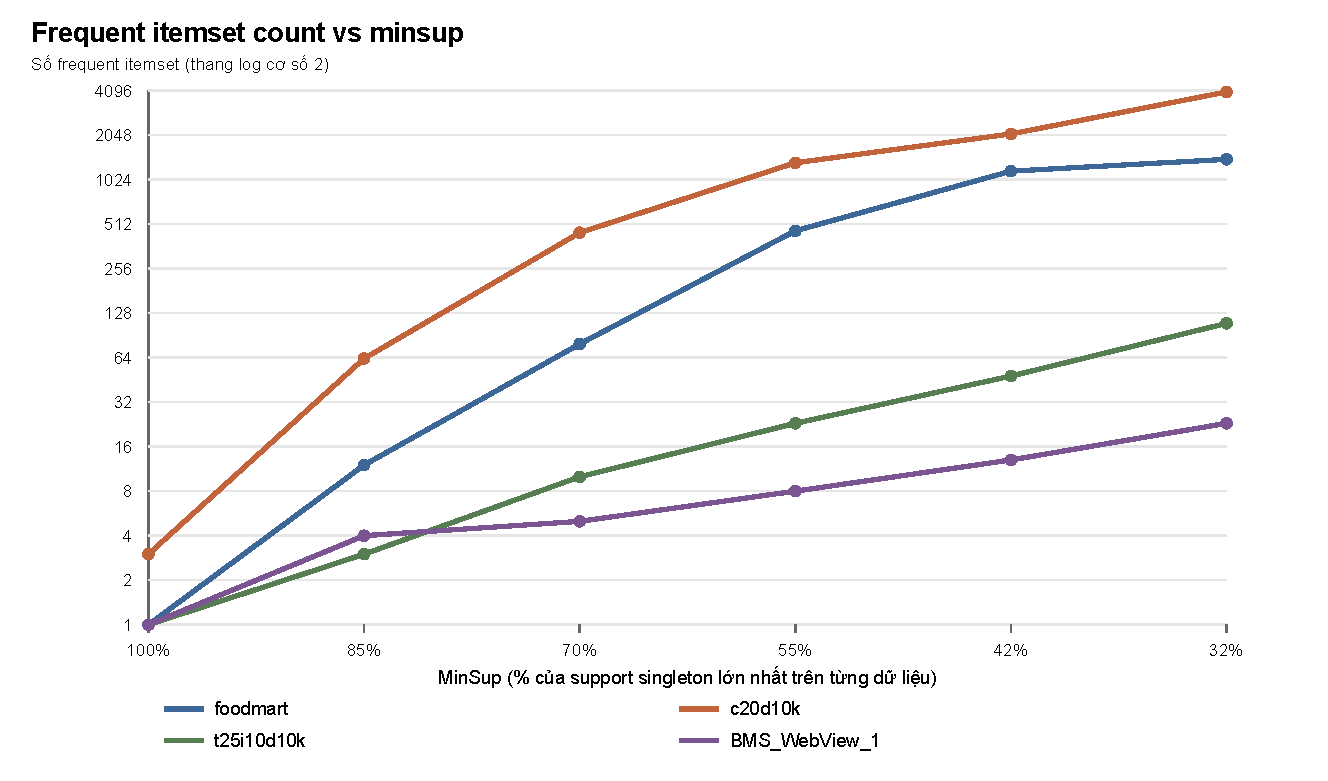
\includegraphics[width=0.82\textwidth]{figures/patterns.pdf}
\caption{Số frequent itemset theo minsup trên bốn bộ benchmark.}
\label{fig:pattern-counts}
\end{figure*}

Khi minsup giảm từ mức cao nhất xuống thấp nhất, số itemset tăng trên cả
bốn bộ: c20d10k từ 3 lên 3999, Foodmart từ 1 lên 1400, t25i10d10k từ 1
lên 109 và BMS\_WebView\_1 từ 1 lên 23. Theo thống kê parser, mật độ giao
dịch ước lượng bằng độ dài giao dịch trung bình chia số item phân biệt lần
lượt xấp xỉ 10.42\% với c20d10k, 2.67\% với t25i10d10k, 0.51\% với
BMS\_WebView\_1 và 0.28\% với Foodmart. Kết quả phù hợp với xu hướng dữ
liệu dày hơn tạo nhiều tổ hợp phổ biến hơn trong các cấu hình đã thử; tuy
nhiên đây không phải quan hệ nhân quả được cô lập, vì số giao dịch, phân
bố item và các ngưỡng support tuyệt đối khác nhau giữa các bộ.

\subsection{Ảnh hưởng của ngưỡng support}

Trên Foodmart, khi ngưỡng support tuyệt đối giảm từ
25 xuống 8, số frequent itemset tăng từ 1 lên 1400.
Thời gian của backend set tăng từ 0.026090 lên
1.021860 giây. Backend bitset tăng từ 0.024859
lên 0.892147 giây. Kết quả cho thấy chi phí khai
thác chịu ảnh hưởng đáng kể bởi số lượng itemset
được tìm thấy, không chỉ bởi kích thước dữ liệu.

\begin{figure*}[!t]
\centering
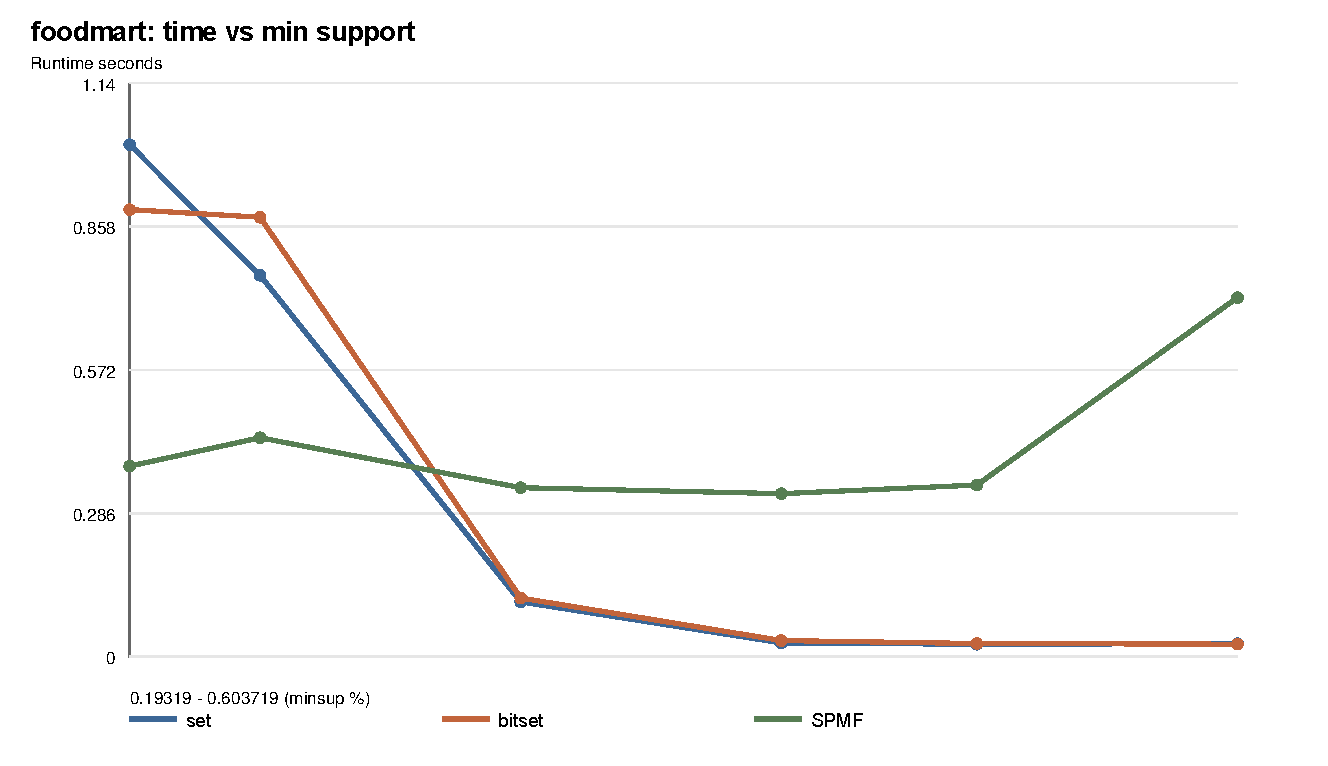
\includegraphics[width=0.85\textwidth]{figures/foodmart.pdf}
\caption{Thời gian chạy Eclat trên Foodmart theo ngưỡng support.}
\label{fig:foodmartreal}
\end{figure*}

\subsection{So sánh TID-set và bitset}

Ở c20d10k với ngưỡng support tuyệt đối 3200,
backend set mất 0.685201 giây, trong khi bitset
mất 0.303265 giây. Như vậy, bitset nhanh khoảng
2.26 lần trong cấu hình này. Tuy nhiên, sự khác
biệt không đồng nhất ở tất cả các ngưỡng,
nên không thể kết luận bitset luôn nhanh hơn.

\begin{figure*}[!t]
\centering
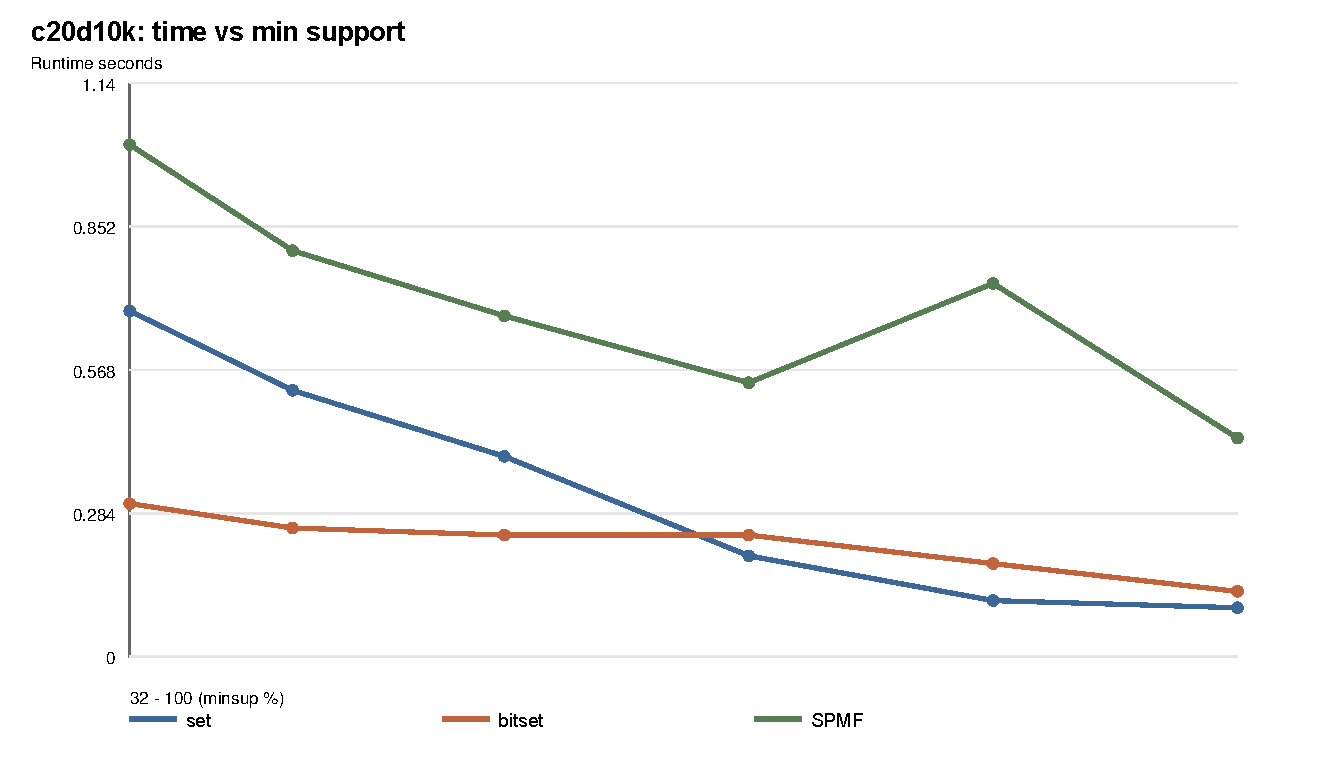
\includegraphics[width=0.85\textwidth]{figures/c20.pdf}
\caption{So sánh thời gian của hai backend trên c20d10k.}
\label{fig:c20real}
\end{figure*}

\subsection{Đặc điểm dữ liệu web thưa}

BMS\_WebView\_1 có 59602 giao dịch và 497 item
khác nhau. Khi minsup giảm từ 3658 xuống 1171
giao dịch, số frequent itemset tăng từ 1 lên 23.
Trong các phép đo đã thực hiện, backend set có
thời gian thấp hơn bitset ở một số ngưỡng,
cho thấy hiệu quả của biểu diễn dữ liệu còn phụ
thuộc vào phân bố giao dịch.

\begin{figure*}[!t]
\centering
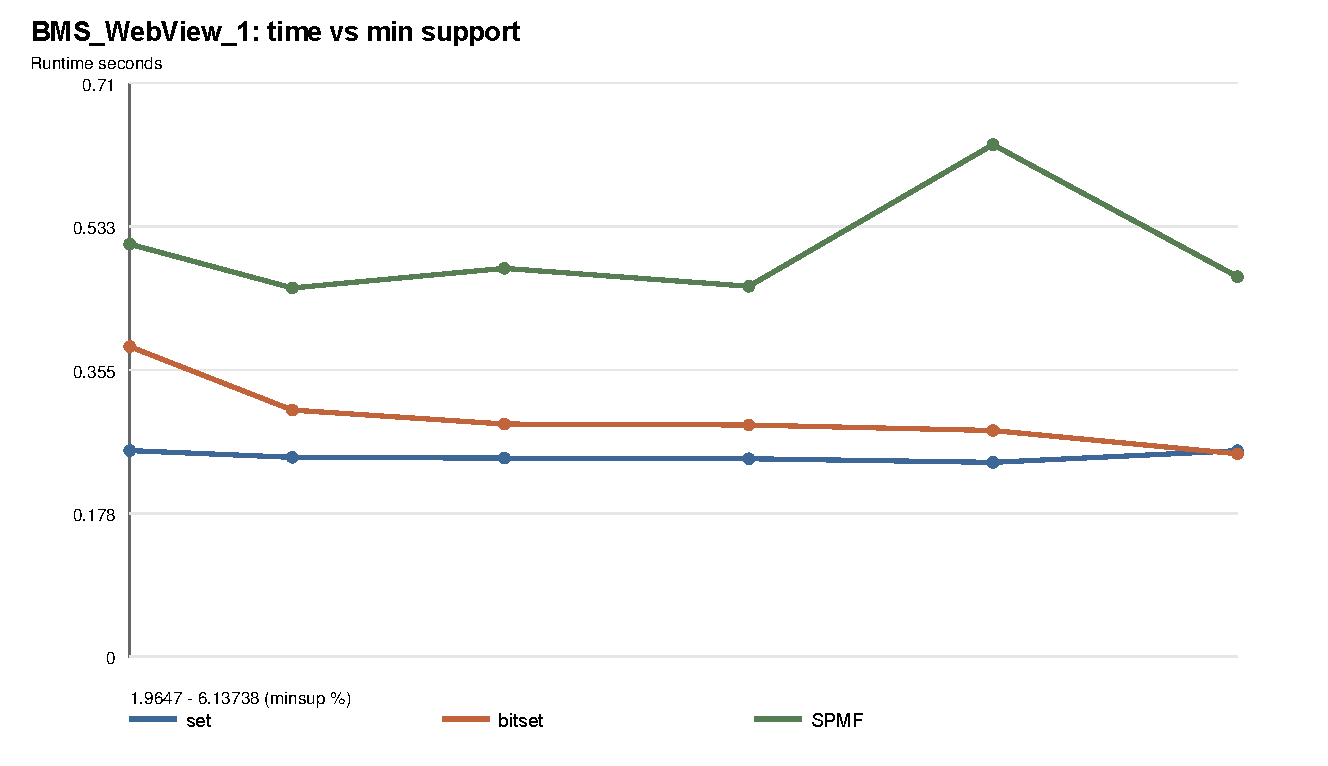
\includegraphics[width=0.85\textwidth]{figures/bms.pdf}
\caption{Thời gian chạy Eclat trên BMS WebView 1.}
\label{fig:bmsreal}
\end{figure*}

\subsection{Đánh giá bộ nhớ}

Biểu đồ bộ nhớ Python của c20d10k đo bằng
tracemalloc, chỉ phản ánh các cấp phát được Python
theo dõi. Phép đo RSS trong tiến trình riêng tại
minsup 5500 ghi nhận 85.2305 MiB với backend set
và 62.8398 MiB với backend bitset. Hai loại phép
đo không được xem là tương đương.

\begin{figure*}[!t]
\centering
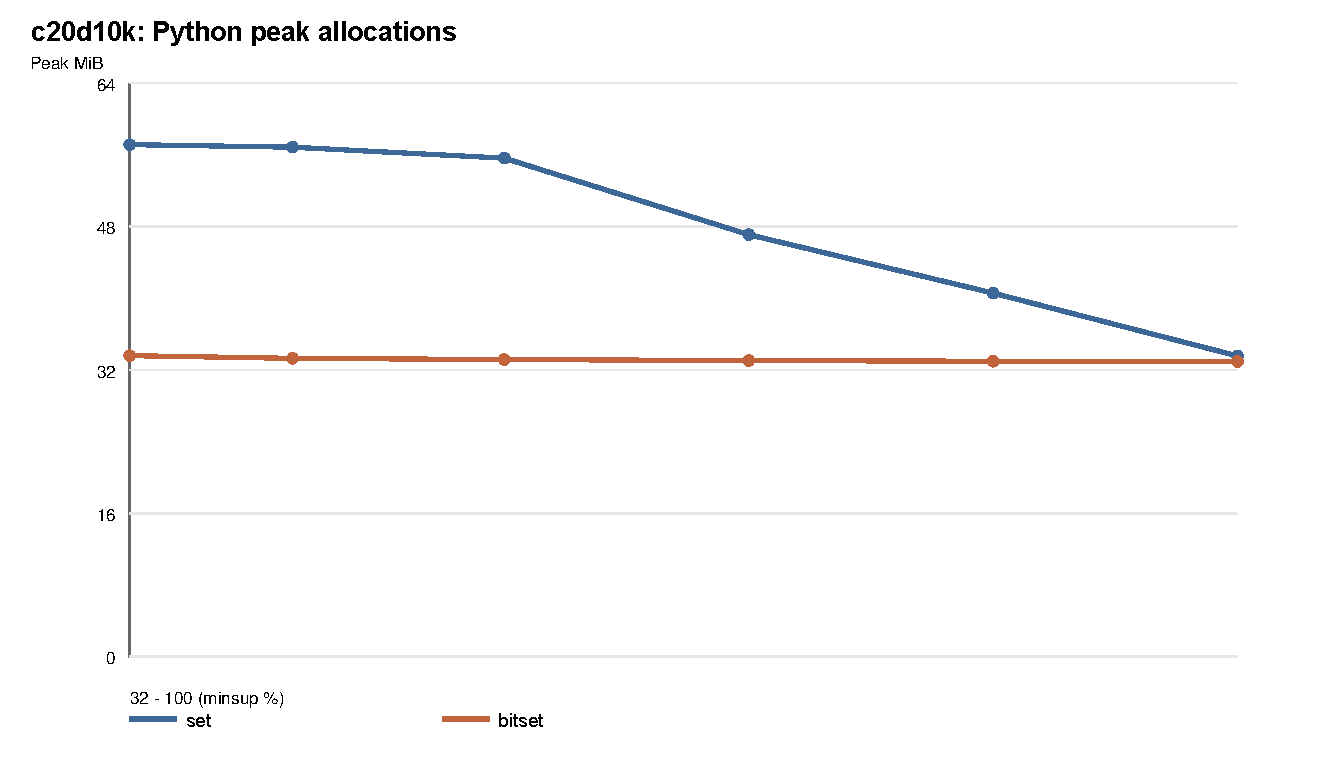
\includegraphics[width=0.85\textwidth]{figures/memory.pdf}
\caption{Bộ nhớ cấp phát Python trên c20d10k, đo bằng tracemalloc.}
\label{fig:memoryreal}
\end{figure*}

\subsection{Khả năng mở rộng}

Thí nghiệm scalability sử dụng lần lượt
10\%, 25\%, 50\%, 75\% và 100\% số giao dịch
của BMS\_WebView\_1. Khi tăng từ 5960 lên
59602 giao dịch, thời gian chạy tăng từ
0.043374 lên 0.472338 giây. Các kết quả
cho thấy xu hướng tăng thời gian theo quy mô
dữ liệu trong cấu hình đã đo, nhưng chưa đủ
để khẳng định một độ phức tạp tiệm cận cụ thể.

\begin{figure*}[!t]
\centering
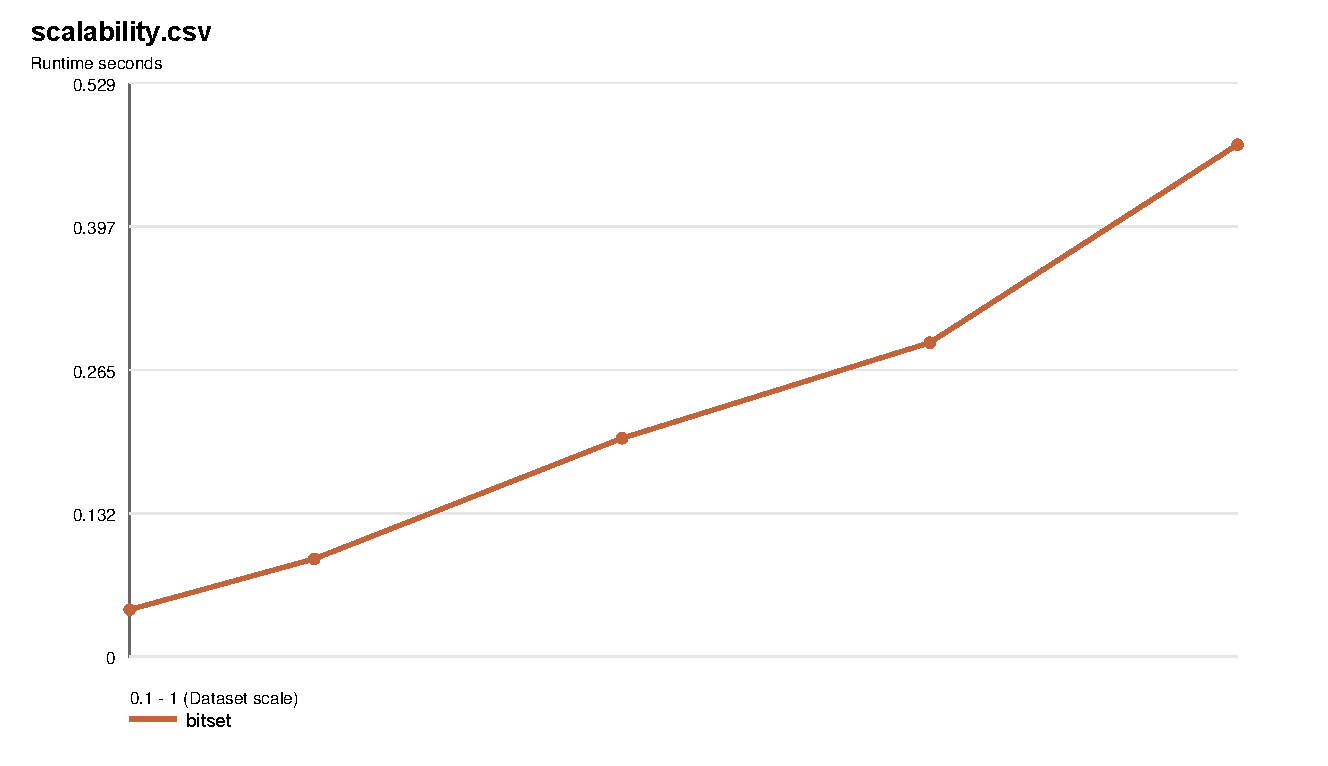
\includegraphics[width=0.85\textwidth]{figures/scalability.pdf}
\caption{Khả năng mở rộng của backend bitset trên BMS WebView 1.}
\label{fig:scalabilityreal}
\end{figure*}

\subsection{Ảnh hưởng của độ dài giao dịch}

Khi độ dài giao dịch trung bình thay đổi từ
3 đến 11 trong bộ dữ liệu tổng hợp, thời gian
chạy ghi nhận lần lượt là 0.009214 và
0.019488 giây ở hai đầu khoảng thử nghiệm.
Số frequent itemset tương ứng tăng từ 52
lên 285. Sự biến thiên này cho thấy độ dài
giao dịch có thể ảnh hưởng đến số tổ hợp
cần xử lý; đồng thời sự thay đổi phân bố
item trong dữ liệu tổng hợp cũng phải được
xem xét khi diễn giải.

\begin{figure*}[!t]
\centering
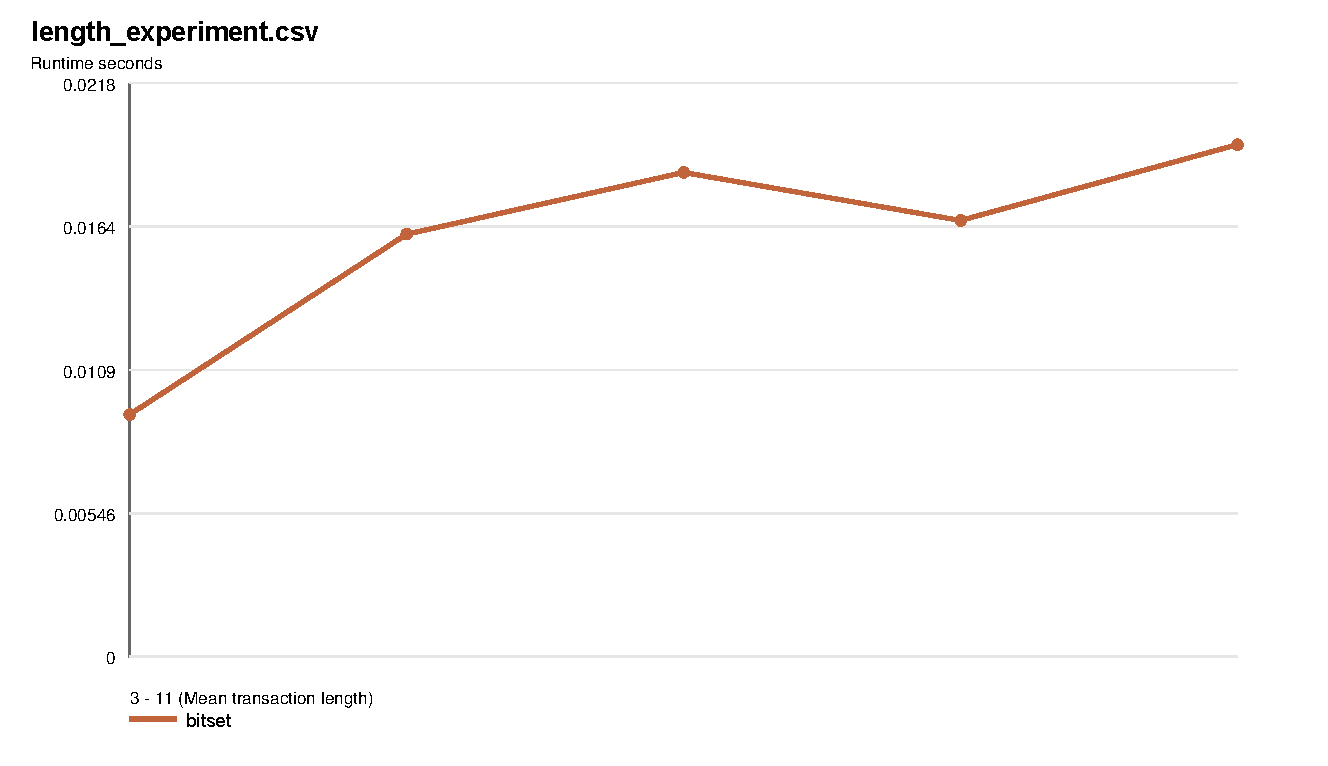
\includegraphics[width=0.85\textwidth]{figures/length.pdf}
\caption{Thời gian chạy theo độ dài giao dịch trong dữ liệu tổng hợp.}
\label{fig:lengthreal}
\end{figure*}

\subsection{Giới hạn của kết quả}

Các thời gian trên là phép đo thực nghiệm
trên môi trường đã sử dụng và chưa được
đại diện bằng trung bình từ nhiều lần chạy.
Thời gian khởi động JVM trong phép chạy SPMF
không thể so sánh trực tiếp với thời gian
khai thác trong tiến trình Python.
Những giới hạn này cần được tính đến khi
đánh giá hiệu năng của Eclat.

\begin{figure*}[!t]
\centering
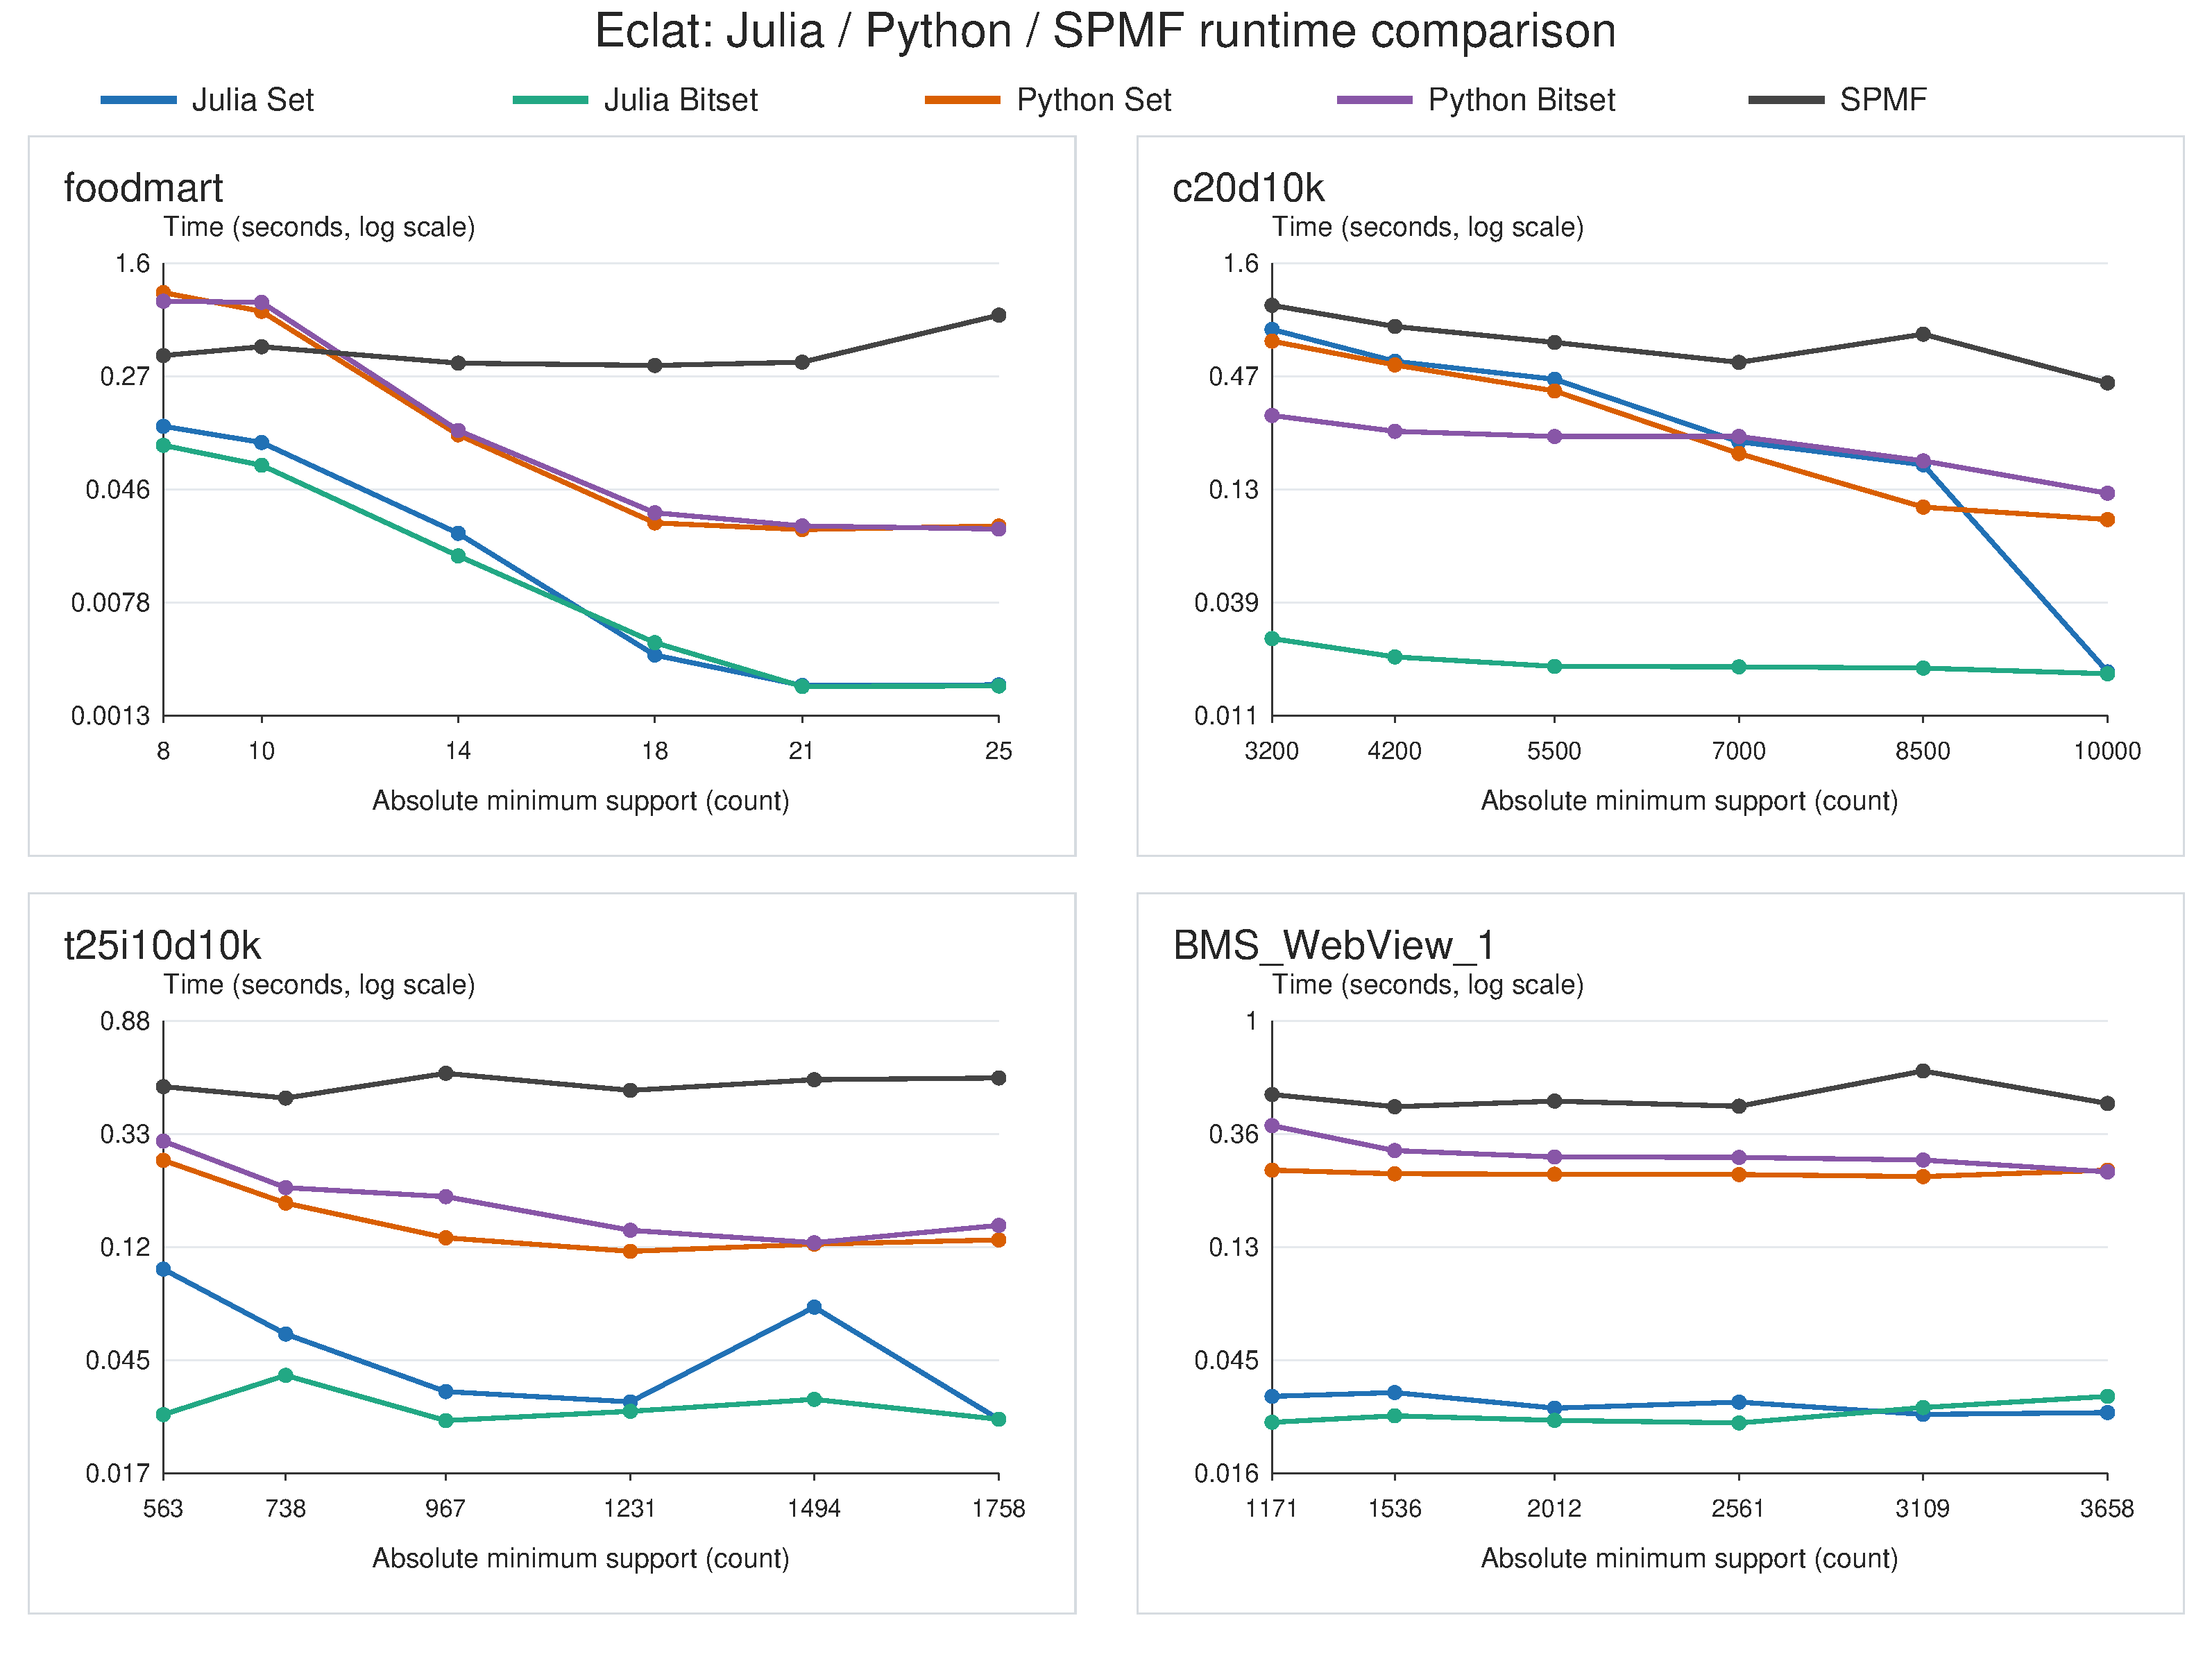
\includegraphics[width=\textwidth]{figures/julia_python_spmf_runtime.pdf}
\caption{Thời gian chạy Eclat trên bốn bộ dữ liệu với sáu mức minimum support: Julia (Set và BitVector), Python (set và bitset), và SPMF. Trục tung dùng thang logarit. Số liệu SPMF bao gồm khởi động JVM, trong khi thời gian Julia/Python được lấy từ benchmark riêng. Các phép đo không phải một so sánh hiệu năng thuần thuật toán trong điều kiện kiểm soát đồng nhất.}
\label{fig:julia-python-spmf-runtime}
\end{figure*}
Hình~\ref{fig:julia-python-spmf-runtime} tổng hợp kết quả thời gian của hai bản cài đặt do nhóm phát triển và SPMF. Mỗi mức support có một phép đo được ghi trong các tệp CSV của phiên chạy dùng để tạo đồ thị. Phần Julia và Python được thực hiện như các benchmark riêng, còn SPMF bao gồm chi phí khởi động JVM. Vì thế đồ thị mô tả số liệu quan sát, không đủ để kết luận tốc độ thuần thuật toán trên các môi trường thực thi khác nhau.

\clearpage
\balance
\section{Tổng kết}
Project đã xây dựng hai bản Eclat độc lập bằng Python và Julia, hỗ trợ TID-set/bitset, giao diện dòng lệnh tương thích SPMF và hai pipeline ứng dụng sử dụng cùng nguyên lý khai thác. Điểm mạnh của cách tổ chức này là tất cả support count và luật kết hợp được sinh bởi code của chính project; mọi dữ liệu thật đều có link đến file nguồn và cơ chế lưu checksum. Về mặt giải thuật, khả năng giao tập giao dịch là trung tâm của Eclat; về mặt triển khai, cả cấp phát bộ nhớ và kích thước output cần được đo thay vì suy luận chỉ từ số dòng dữ liệu.

Các thí nghiệm đã hoàn thành 48 lượt benchmark Python và 48 lượt benchmark Julia trên bốn bộ dữ liệu. Julia đạt 77/77 phép kiểm thử; cả hai bản cài đặt đều đạt 24/24 phép đối chiếu benchmark với SPMF theo từng itemset và support. Riêng lần chạy Python trên Colab có thêm một dữ liệu toy, đạt 25/25. Trên BMS\_WebView\_1, mã item được ánh xạ tạm thời về miền 1 đến 497 khi gọi SPMF nhằm tránh cấp phát ma trận quá lớn; kết quả sau đó được đổi về mã gốc để so sánh. Tệp dữ liệu gốc không bị thay đổi.

Thí nghiệm scalability cho thấy khi tăng số giao dịch từ 5,960 lên 59,602, thời gian chạy bitset tăng từ 0.043374 lên 0.472338 giây. Ứng dụng giỏ hàng sinh được top-10 luật theo lift; ứng dụng hình ảnh tạo codebook gồm 12 visual words từ 600 ảnh và khai thác được 37 mẫu. Kết quả cho thấy Eclat có thể áp dụng cho nhiều dạng dữ liệu sau bước chuyển đổi phù hợp. Tuy nhiên, các phép đo thời gian đơn lẻ còn chịu ảnh hưởng của hệ thống, còn biểu diễn bag-of-visual-words làm mất thông tin vị trí. Các hướng cải tiến tiếp theo là giảm chi phí phép giao trên dữ liệu thưa, lặp lại benchmark trong cùng môi trường cho so sánh công bằng và đánh giá đặc trưng ảnh trên tác vụ downstream.
\begin{thebibliography}{99}
\bibitem{zaki2000} M. J. Zaki, ``Scalable Algorithms for Association Mining,'' \emph{IEEE Trans. Knowl. Data Eng.}, vol. 12, no. 3, pp. 372--390, 2000. doi: 10.1109/69.846291.
\bibitem{agrawal1994} R. Agrawal and R. Srikant, ``Fast Algorithms for Mining Association Rules in Large Databases,'' \emph{Proc. VLDB}, pp. 487--499, 1994.
\bibitem{fournier2016} P. Fournier-Viger \emph{et al.}, ``The SPMF Open-Source Data Mining Library Version 2,'' \emph{PKDD/ECML Workshop on Machine Learning and Data Mining for Sports Analytics}, 2016.
\bibitem{sivic2003} J. Sivic and A. Zisserman, ``Video Google: A Text Retrieval Approach to Object Matching in Videos,'' \emph{Proc. IEEE ICCV}, 2003, doi: 10.1109/ICCV.2003.1238663.
\bibitem{ucidigits} UCI Machine Learning Repository, ``Optical Recognition of Handwritten Digits,'' \url{https://archive.ics.uci.edu/dataset/80/optical+recognition+of+handwritten+digits}.
\bibitem{spmfdata} SPMF, ``Public Datasets,'' \url{https://www.philippe-fournier-viger.com/spmf/index.php?link=datasets.php}.
\bibitem{assignment} HCMUS Course Lab Book, ``Khai thác tập phổ biến,'' \url{https://hcmus-cs-ta.github.io/lab-book/data-mining/projects/itemset/}.
\end{thebibliography}
\end{document}
